\documentclass[journal]{IEEEtran}
\usepackage[T1]{fontenc}
\usepackage{newtxtext,newtxmath}
\usepackage{amsmath,mathtools}
\usepackage{booktabs,array,tabularx,multirow}
\usepackage{graphicx}
\graphicspath{{figures/}}
\usepackage{xcolor}
\usepackage{cite}
\usepackage{url}
\usepackage{hyperref}
\hypersetup{hidelinks}
\usepackage{enumitem}
\setlist{nosep,leftmargin=*}
\usepackage{microtype}
\usepackage{balance}

\newtheorem{proposition}{Proposition}
\newtheorem{lemma}{Lemma}
\newtheorem{definition}{Definition}
\newenvironment{proof}{\par\noindent\textit{Proof.} }{\hfill$\square$\par}
\newcommand{\Self}{\mathrm{Self}}
\newcommand{\Tool}{\mathrm{Tool}}
\newcommand{\Object}{\mathrm{Object}}
\newcommand{\Agent}{\mathrm{Agent}}
\newcommand{\CIAS}{\textsc{CIAS}}
\newcommand{\argmin}{\operatorname*{arg\,min}}
\newcommand{\argmax}{\operatorname*{arg\,max}}

\title{A Causal Theory of Persistent Functional Self in Embodied Artificial Agents}

\author{Mykola~Shatokhin%
\thanks{Mykola Shatokhin is a Ph.D. student with the Faculty of Computer Science and Technologies, National University ``Kyiv Aviation Institute'', Kyiv, Ukraine (e-mail: n.shatokhin@gmail.com; ORCID: 0000-0003-0028-6208).}%
\thanks{Corresponding author: Mykola Shatokhin (e-mail: n.shatokhin@gmail.com).}}

\begin{document}
\maketitle

\begin{abstract}
Embodied agents are usually given a privileged identity: their sensors, actuators, body, and memory are labeled as ``self'' by design. We study identity preservation when appearance and position become unreliable. Persistent functional Self is modeled as causal individuation, embodied closure, and a compact cross-change identity anchor. In a controlled 240-frame sensorimotor benchmark, the true body is transformed and relocated while an old-looking lure remains near the previous location and receives partially plausible false causal cues. The experiment uses engineered semantic causal-role variables; learning features from raw sensory streams is outside the present experiment. After an initial ceiling-prone diagnostic and a repaired matched diagnostic, scientific behavior, endpoint definitions, thresholds, and seed ranges were frozen. In a fresh 360-run confirmatory rerun, Full scored $Q=0.883$ versus $0.410$ after selective anchor lesion, with paired $\Delta Q=+0.473$ (95\% CI $[0.416,0.531]$, $d_z=3.08$). Lure capture was $0.035$ versus $0.775$, a rejection advantage of $+0.740$ ($[0.653,0.828]$, $d_z=3.16$). A separate supervised generic recurrent estimator, fit only on diagnostic seeds and lacking an explicit Self role, lineage key, or reconnect rule, slightly exceeded CIAS Full on a disjoint held-out set: Full-minus-generic was $-0.051$ for identity continuity and $-0.022$ for lure rejection. The selected estimator used zero additional appearance-continuity penalty, although appearance components remained in its diagnostic-fitted emission model. A 27-setting sensitivity experiment on another held-out seed range preserved both Full-versus-lesion effect signs with positive pointwise 95\% intervals in 25/27 settings; a family-wise max-bootstrap interval across all 54 sensitivity effects retained both positive lower bounds in 24/27 settings. These results establish the CIAS anchor as an effective architecture-specific mechanism and show that a generic recurrent state estimator can solve the same structured benchmark without an explicit Self anchor. Phenomenal consciousness is outside the claims of this study.
\end{abstract}

\begin{IEEEkeywords}
artificial self, embodied AI, persistent identity, causal inference, cognitive robotics, reproducibility
\end{IEEEkeywords}

\section{Introduction}
\IEEEPARstart{A}{utonomous} agents increasingly learn over long horizons, recover from damage, and move between tasks or hardware configurations. Yet most artificial systems receive a privileged answer to a question that biological agents must solve: which observed entity is me? A controller typically knows which joint vector is ``its'' proprioception, which camera is ``its'' camera, and which object identifier denotes ``its'' body. These abstractions are useful engineering conveniences. Persistent agents still require a mechanism that answers a separate question: how can identity remain stable when the body is altered, relocated, visually transformed, or partially mimicked by another entity?

Human self-research separates agency, body ownership, and temporal/autobiographical selfhood \cite{Gallagher2000,Braun2018,Blanke2015,Conway2000}; multisensory and predictive accounts further emphasize relations among vision, proprioception, touch, and interoception as determinants of bodily ownership \cite{Botvinick1998,Tsakiris2010,Seth2013,Apps2014}. Robotics has operationalized several relevant components: continuous self-modeling for damage adaptation \cite{Bongard2006}, sensorimotor self-perception on physical robots \cite{Lanillos2017,Oliver2022}, developmental accounts of an artificial minimal self \cite{Hafner2020,Forch2021}, self/other distinction from sensorimotor contingency \cite{Lanillos2020,Chen2026}, learned egocentric body dynamics \cite{Hu2025}, and broad integrated self-model frameworks \cite{Jiang2026}. These works motivate a multifactorial treatment of Self. The present study isolates the narrower problem of temporal identity across embodiment change.

Persistent identity is also a state-estimation and data-association problem. Classical alternatives include linear state-space filtering \cite{Kalman1960}, hidden-state sequence models \cite{Rabiner1989}, and POMDP belief-state estimation \cite{Kaelbling1998}; modern tracking systems preserve object identity through learned association metrics or transformer state \cite{Wojke2017,Luo2021,Meinhardt2022}. These methods are important competitors because none requires a variable named ``Self.'' We therefore supplement the within-CIAS lesion with an independent recurrent state estimator that receives the same model-visible observation stream, is fit only on diagnostic seeds, and contains no explicit Self role, persistent lineage key, or change-point reconnect rule.

We ask whether one inferred entity can remain the same functional subject when appearance and position become misleading. Our hypothesis is that \emph{persistent functional identity is better represented by causal continuity than by current appearance similarity}. Here, ``functional'' denotes a computational subject variable. Phenomenal experience is outside the scope of the experiment.

The paper makes five contributions. First, it formalizes persistent functional Self as causal individuation, embodied closure, and persistent cross-change identity state. Second, it provides an adversarial benchmark in which the current body is transformed while a previous-looking competitor remains present. Third, it reports the complete diagnostic-to-confirmatory methodology and explicitly defines pilot, freeze, preflight, seed, run, and held-out evidence. Fourth, it separates the \emph{form} of the theory from the hand-designed numerical instantiation and explains the provenance of the confirmatory equations. Fifth, it tests architectural specificity with a generic recurrent estimator and evaluates mechanism robustness across 27 prespecified parameter settings on fresh held-out seeds.

\section{Operational Problem and Terminology}
At time $t$, the simulated agent receives observations
\begin{equation}
\mathcal O_t=\{o_{1,t},\ldots,o_{n_t,t}\}.
\label{eq:observations}
\end{equation}
Equation~\eqref{eq:observations} defines the benchmark bookkeeping. The world is represented as a set because several candidate entities can be visible in the same frame and their order is intentionally shuffled. Each observation contains position, an appearance/signature vector, and causal-role features. The identity-relevant feature vector is
\begin{equation}
\phi(o)=(m,p,\tau,\chi,i,h,a,\ldots),
\label{eq:features}
\end{equation}
where $m$ is motor-authorship evidence, $p$ proprioceptive closure, $\tau$ temporal match, $\chi$ cross-modal coherence, $i$ interoceptive closure, $h$ homeostatic coupling, and $a$ action-history match. The experiment uses engineered semantic signals and therefore evaluates identity maintenance after informative causal-role variables are available. Learning those variables from pixels, tactile arrays, or raw interoceptive streams is a separate causal-representation-learning problem \cite{Scholkopf2021} outside the present test.

The ontology maintains latent entities
\begin{equation}
\mathcal E_t=\{e_1,\ldots,e_{k_t}\}
\label{eq:entities}
\end{equation}
and infers which current observation belongs to which existing entity. The Self is represented as a role hypothesis assigned to an inferred entity; the environment supplies no privileged Self object identifier.

\begin{definition}[Persistent functional Self]
A persistent functional Self is a lineage $S_{1:T}$ of latent entities for which self-specific causal evidence remains high relative to competitors and whose identity can remain invariant across a declared change point despite a discontinuity in current appearance or position.
\end{definition}

A \emph{change point} is a declared regime transition at which appearance, position, and morphology may become unreliable while causal lineage can persist. The change-point marker does not itself assign a new identity. A \emph{lure} is a competing external entity made deliberately similar to the previous Self. An \emph{embodiment profile} specifies a synthetic reliability/noise regime; the four profiles are not physical robots.

\section{Theory, Equations, and Parameter Provenance}
\subsection{How to read the equations}
The equations use three classes of quantities with different scientific status.

\begin{enumerate}
\item \textbf{Theory structure:} which relations matter---for example, identity association must combine appearance, predicted position, and causal-role dynamics; Self evidence must be multifactorial; a change point requires a lineage-transfer mechanism.
\item \textbf{Implementation parameters:} numerical weights, smoothing rates, and thresholds used by the tested implementation. These values were chosen by hand during exploratory development to realize qualitative constraints and obtain a usable, nondegenerate mechanism. They are neither fitted biological coefficients nor universal constants of Self.
\item \textbf{Evaluation parameters:} weights and thresholds in the benchmark endpoint and confirmatory decision rule. They define what counted as success; after diagnostics they were fixed before confirmatory data were opened.
\end{enumerate}

The held-out experiment tests one \emph{frozen instantiation} of the theory. Theory motivates the cue families, signs, relative priorities, and post-change shift. Values such as 0.43 or 2.70 specify the reproducible engineering operating point used for confirmation; the experiment does not estimate parameter uniqueness or optimality.

\subsection{How the mathematical form emerged}
The equations encode a sequence of design constraints and negative results. First, Self could not be represented by a privileged object identifier, which required a latent entity-association problem. Second, a single action-contingency cue could also describe a controlled tool, which motivated a multifactorial role vector combining motor, proprioceptive, interoceptive, homeostatic, temporal, and history evidence. Third, unconstrained continuity heuristics in earlier development could merge distinct entities, motivating the one-to-one assignment in Eq.~\eqref{eq:assignment}. Fourth, radical body change makes appearance and local position unreliable exactly when continuity matters most, motivating the post-change reweighting and a separate causal identity anchor. Finally, the first adversarial diagnostic drove a simple retention metric to a ceiling, motivating the multi-component endpoint in Eq.~\eqref{eq:q}. Thus the form of the model is traceable to specific identifiability and measurement problems, whereas the exact numerical coefficients remain one frozen implementation.

\subsection{Motor authorship as a cue conjunction}
Motor authorship is
\begin{equation}
m(o)=\sqrt{\max(0,e(o)y(o))},
\label{eq:motor}
\end{equation}
where $e$ is efference-copy evidence and $y$ is action-outcome match. The form is a geometric conjunction: high motor authorship requires both evidence that an action was issued and evidence that the observed consequence matches it. If either factor vanishes, authorship vanishes. The square root keeps the result on approximately the same $[0,1]$ scale as its inputs instead of shrinking two moderate cues by an uncorrected product. This equation specifies the model design; no psychophysical fit was used to obtain it.

\subsection{Entity association as causal individuation}
Observation $o_i$ is matched to entity $e_j$ by the multi-cue cost
\begin{equation}
C_{ij}=w_s d_s(o_i,e_j)+w_x d_x(o_i,e_j)+w_\phi d_\phi(o_i,e_j)+c_{\rm age},
\label{eq:assoc}
\end{equation}
where $d_s$ is normalized signature distance, $d_x$ predicted-position distance, $d_\phi$ distance between causal-role feature vectors, and $c_{\rm age}$ penalizes stale entities. This is the standard engineering logic of multi-cue data association: no single cue is trusted absolutely, so commensurate distances are combined into one matching cost.

During ordinary continuity, the implementation uses
\begin{equation}
(w_s,w_x,w_\phi)=(0.43,0.37,0.20).
\label{eq:normalweights}
\end{equation}
The three weights sum to one and favor appearance and local motion because these are efficient identity cues away from a declared discontinuity. After a change point, the structural equation is retained with the weights
\begin{equation}
(w_s,w_x,w_\phi)=(0.20,0.29,0.51),
\label{eq:cpweights}
\end{equation}
so causal-role dynamics receive the majority weight. The qualitative reason is theoretical: the experiment deliberately invalidates old appearance at a change point, so an identity mechanism that continues to privilege appearance would be structurally biased toward the lure. The exact decimals are hand-designed implementation parameters chosen before confirmatory testing; no likelihood fit was used to obtain them.

Assignments are one-to-one and minimize total cost,
\begin{equation}
\pi_t^*=\argmin_{\pi\in\Pi}\sum_i C_{i,\pi(i)},
\label{eq:assignment}
\end{equation}
implemented with the Hungarian assignment algorithm \cite{Kuhn1955,Munkres1957}. The one-to-one constraint is conceptually important: one current observation cannot simultaneously inherit multiple old identities, and one old entity cannot be assigned to several visible bodies. This constraint was introduced during the broader research program after unconstrained continuity heuristics were found capable of merging distinct entities.

\subsection{Temporal smoothing and role scores}
Each entity carries temporally smoothed causal features. For a generic feature $z$ observed as $\tilde z_t$,
\begin{equation}
z_t=(1-\alpha)z_{t-1}+\alpha\tilde z_t,\qquad \alpha=0.12.
\label{eq:ewma}
\end{equation}
This exponential smoothing represents each cue as a short temporal history across frames. At the benchmark step of $0.1$~s, $\alpha=0.12$ corresponds to a contribution half-life of about $5.4$ frames ($0.54$~s). The value is an engineering compromise between stability and adaptation. The held-out experiment evaluates this fixed choice; parameter optimality was not estimated.

A role energy is then a signed linear evidence score. For Self,
\begin{equation}
\begin{aligned}
E_{\Self}={}&2.70m+1.90p+0.90\tau+0.55\chi+0.35r \\
&+1.55i+1.25h+0.95a-1.35u-0.75q-1.75\ell.
\end{aligned}
\label{eq:selfenergy}
\end{equation}
where $r$ is persistence, $u$ autonomous external dynamics, $q$ other-agent-like response contingency, and $\ell$ tool coupling. Positive coefficients encode evidence expected of one's own body; negative coefficients encode patterns more characteristic of an independently acting entity or a tool. Motor authorship and proprioception receive large positive Self weights; tool coupling is strongly negative for Self. The complete Tool/Object/Agent score equations and coefficient-by-coefficient interpretation are given in the Supplementary Material.

The four energies are normalized by
\begin{equation}
P(R=r\mid e)=\frac{\exp(E_r)}{\sum_{k\in\{\Self,\Tool,\Object,\Agent\}}\exp(E_k)}.
\label{eq:softmax}
\end{equation}
Softmax is used because the roles compete and a normalized relative score is convenient for subsequent decisions. We retain the notation $P$ for compatibility with the implementation. These quantities are \emph{operational normalized role scores}; no calibration to Bayesian posteriors from population data was performed.

\subsection{Persistent causal identity anchor}
Immediately before a change point, the mechanism stores the most Self-like entity. Current observation-level causal closure is summarized by
\begin{equation}
A_o=0.26m+0.18p+0.24i+0.18h+0.14a,
\label{eq:ao}
\end{equation}
and the pre-change entity-level anchor by
\begin{equation}
A_e=0.26P(\Self)+0.18m_e+0.14p_e+0.18i_e+0.14h_e+0.10a_e.
\label{eq:ae}
\end{equation}
Both are convex combinations: their coefficients sum to one. The observation anchor deliberately excludes appearance and absolute position because those are precisely the cues that can fail at a body transfer. Motor authorship and interoceptive closure receive the largest observation weights; the entity-level anchor additionally includes the accumulated Self-role score. The exact proportions are hand-designed and were frozen before confirmation.

Let $e^*=\argmax_e A_e$ be the pre-change lineage candidate. If a post-change observation has $A_o>0.70$ and is assigned to $e^*$, its cost is replaced by
\begin{equation}
C_{\rm anchor}=0.015+0.06(1-A_o)+0.04(1-A_e).
\label{eq:anchorcost}
\end{equation}
This form converts strong present closure and strong stored identity into a very cheap reconnection edge. The small positive baseline prevents a mathematically perfect zero-cost edge; the residual terms make the cost increase as current or stored evidence weakens. Conversely, assigning the same high-anchor observation to a nonpersistent entity incurs an additional $2A_o$ penalty. These numbers were selected to create a clear separation around a change point while preserving defeasibility as causal evidence weakens. They are auditable mechanism constants and carry no claimed psychological calibration. The post-change association threshold is $0.82$; its role is to allow a wider matching window than the ordinary $0.66$ threshold while still rejecting grossly incompatible entities.

\noindent\emph{Identifiability sanity check.}
Suppose two hypotheses exchange which of two bodies carries the persistent lineage while inducing the same appearance likelihood and equal priors. Bayes' rule then gives equal posterior probability to the two hypotheses, so an appearance-only estimator cannot prefer the correct lineage above chance in expectation. This elementary identifiability observation motivates the benchmark design: appearance alone cannot identify the persistent lineage under the stated symmetry assumptions.

The benchmark uses an asymmetric adversarial case: the lure is \emph{more similar} to the old appearance and old location than the transformed true Self.

\section{Experimental Program}
\subsection{What happens in one run?}
The confirmatory benchmark is a controlled identity experiment. Each run uses sensorimotor probing to generate evidence for entity identity; navigation, foraging, and manipulation rewards are absent.

One run lasts 240 simulation frames with $\Delta t=0.1$~s, i.e., 24 simulated seconds. It contains four 42-frame exposure blocks followed by a 72-frame adversarial final probe (Fig.~\ref{fig:timeline}). Between exposure blocks, and once more before the final probe, a change point is issued. Thus every confirmatory run contains exactly four change-point events.

\begin{figure}[t]
\centering
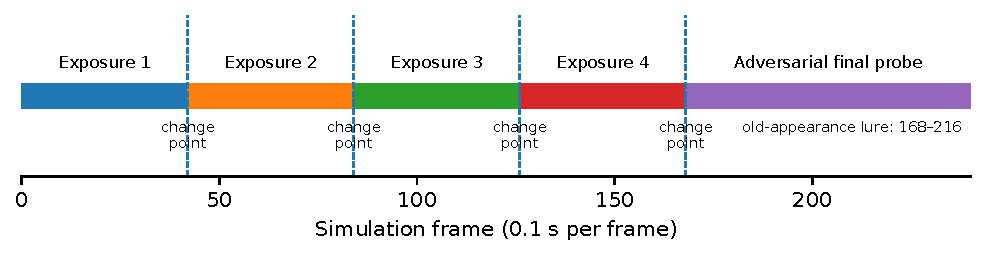
\includegraphics[width=\columnwidth]{run_timeline.pdf}
\caption{Lifecycle of one run. The agent performs continuous sensorimotor activity throughout. A change point separates each exposure block; an old-appearance lure is present for the first 20 frames after intermediate changes and for the first 48 frames of the 72-frame final probe.}
\label{fig:timeline}
\end{figure}

At every frame the benchmark generates an abstract motor-command strength, registers that action in the ontology, moves the true Self along a reproducible oscillatory trajectory around the current body anchor, and emits an observation containing the action-related and body-related cues in Eq.~\eqref{eq:features}. The scene also contains a stable generic object and a generic autonomous agent. Observations are shuffled before association, preventing the Self from being identified by list position.

The control policy and ontology equations remain fixed throughout the four exposure blocks. These blocks provide \emph{sensorimotor exposure}: the latent entity records accumulate temporal, action, body, and role evidence while the embodiment signature and cue reliability vary. In the progressive schedule the abstract morphology level changes from 0 to 1 to 2 to 3. These levels alter the visual signature and the quality/noise of causal signals; they do not represent four fully simulated mechanical robots with task-specific locomotion controllers.

After each intermediate change point, an old-looking clone is temporarily placed near the previous body anchor. The clone is an external Object in ground truth, but it preserves the preceding visual signature and receives partially plausible, action-correlated short-term cues. Simultaneously, genuine Self cues are deliberately intermittent during an ambiguity interval. The final probe strengthens this conflict: the true Self is moved to a new location, its signature is strongly transformed, the old-looking clone remains near the former location for 48 frames, and true causal evidence is imperfect throughout the 72-frame probe. The measured outcome is which visible entity inherits the prior Self lineage when visual continuity and multichannel causal continuity disagree.

\subsection{Seed, run, profile, and condition}
A \emph{seed} is an integer reproducibility key for the deterministic/pseudorandom scenario generator. It controls reproducible geometric anchors, phases, cue perturbations, and schedule choices. It is not an experimental stage, a body, or a learned memory. A \emph{run} is one complete execution for one
\begin{equation}
\text{seed}\times\text{embodiment profile}\times\text{experimental condition}.
\label{eq:runcell}
\end{equation}
Equation~\eqref{eq:runcell} is the factorial definition of an experimental cell. Conditions with the same seed and profile therefore face homologous seed-indexed scenarios and can be compared as paired observations. The pseudorandom stream is deterministic and condition-specific. Pairing therefore refers to homologous seed-indexed scenarios, not byte-identical frame noise.

Four embodiment profiles are used: ground creature, wheeled robot, drone, and virtual avatar. They are controlled regimes of causal reliability and noise, chosen to test whether the mechanism depends on one favorable signal quality. Hardware validation is outside the scope of these four simulated profiles.

The confirmatory experiment compares three conditions: (i) the \emph{Full model}, with the persistent identity anchor enabled; (ii) a \emph{persistent-anchor lesion}, which selectively removes cross-change-point persistent anchoring; and (iii) a \emph{history-reset control}, which clears accumulated entity history at transitions while retaining the post-change association mechanism. The third condition tests whether identity requires retention of all association history. It is excluded from the primary confirmatory pass/fail rule.

\subsection{Why pilot, freeze, preflight, and held-out are separate}
Table~\ref{tab:stages} gives the mission of each methodological stage. These terms describe evidence status, not software versions.

\begin{table*}[t]
\caption{Meaning and scientific mission of the experimental stages.}
\label{tab:stages}
\centering
\footnotesize
\begin{tabularx}{\textwidth}{@{}p{0.14\textwidth}p{0.27\textwidth}p{0.27\textwidth}X@{}}
\toprule
Stage & Mission & What is allowed & Evidential status \\
\midrule
Diagnostic pilot & Find failure modes in the mechanism, benchmark, endpoint, or comparison design. & Inspect outputs; repair code; alter cue schedules, endpoint definitions, and parameters if defects are discovered. & Exploratory only; cannot be used as final confirmation because design choices may depend on these data. \\
Matched diagnostic & Re-run the repaired design on fresh seeds, remove known confounds, and decide which hypotheses remain scientifically defensible. & Further repair is allowed; any change keeps the result in diagnostic status. & Used for theory reduction and specification of the freeze; excluded from final held-out evidence. \\
Scientific freeze & Create the precommitment boundary. & No subsequent change to behavior-affecting scientific code, cue schedule, coefficient values, endpoint formula, pass/fail thresholds, primary claim, or reserved confirmatory seed range. & Methodological boundary with no experimental observations; after this point confirmatory data cannot influence the tested specification. \\
Preflight & Verify that the frozen machinery works on a small fresh sample before spending/opening the main held-out set. & Only operational failures may stop the run; a desired Full-vs-lesion effect is explicitly not required for passage. & Quality-control gate, not confirmatory evidence. \\
Held-out confirmation & Test the frozen hypothesis on untouched seeds not used for model or benchmark design. & No scientific tuning. Results are analyzed with the already-fixed endpoint and decision rule. & Primary inferential evidence. \\
\bottomrule
\end{tabularx}
\end{table*}

The first diagnostic used 8 fresh seeds, four profiles, and six exploratory conditions (192 runs). It revealed an exact ceiling on the original primary endpoint and a confound: morphology-transition conditions had received change-point exposure that a final-body-from-start control had not. The result was retained as a failure diagnosis, not confirmation.

A repaired matched diagnostic used 12 new seeds (288 runs). Every curriculum arm received matched change-point exposure, all curriculum-order controls ended in the same terminal body, history reset used an epoch-aware identity namespace, the old-looking lure received causally plausible cues in addition to its visual match, and the continuity endpoint was replaced by the nondegenerate composite defined below. The persistent-anchor lesion remained strongly impaired, whereas progressive morphology order did not outperform final-from-start, reverse, or random order. The final claim was therefore narrowed before freeze.

After freeze, a 48-run preflight used four new seeds across four profiles and three confirmatory conditions. Its mission was mechanical: complete factorial output, the intended four change points, no missing/duplicate cells, and a nondegenerate endpoint. It passed. Only then were 30 untouched held-out seeds opened, yielding
\begin{equation}
30\;\text{seeds}\times4\;\text{profiles}\times3\;\text{conditions}=360\;\text{runs}.
\label{eq:heldoutcount}
\end{equation}

\subsection{Primary endpoint: what it measures and why}
The initial diagnostic showed that pure discrete lineage retention could saturate at a ceiling. The revised endpoint therefore combines distinct ways identity can succeed or fail:
\begin{equation}
Q=0.30R+0.20(1-L)+0.16G+0.24P+0.10F.
\label{eq:q}
\end{equation}
The five weights sum to one. $R$ is the fraction of final-probe frames that retain the pre-change lineage. $L$ is the fraction of lure-present frames in which the old-looking clone captures that lineage, so $1-L$ rewards lure rejection. Recovery speed is
\begin{equation}
G=\begin{cases}
\exp(-T_{\rm rec}/2.8),&\text{if recovery occurs},\\
0,&\text{otherwise},
\end{cases}
\label{eq:recovery}
\end{equation}
where recovery requires five consecutive correct-lineage frames and $T_{\rm rec}$ is time to the first frame of that stable recovery. The 2.8~s denominator is an engineered time constant that converts latency into a smooth $[0,1]$ reward; it is not a biological timescale.

$P$ is a $[0,1]$ rescaling of the average difference between the true body's Self-role score and the lure's Self-role score. It provides continuous information even when the discrete identity key changes. Fragmentation is penalized by
\begin{equation}
F=\frac{1}{1+0.28(n_{\rm frag}-1)},
\label{eq:fragment}
\end{equation}
where $n_{\rm frag}$ is the number of distinct identity keys used during the final probe. The coefficient 0.28 controls how rapidly extra identities reduce the term.

The endpoint weights are part of the evaluation design; model fitting does not determine them. They were chosen to cover distinct failure modes: retention receives the largest single weight, posterior preference and lure rejection ensure that a superficially stable but wrong identity is penalized, recovery captures transient failure, and fragmentation prevents repeated identity splitting from being ignored. These weights and the 2.8/0.28 scales were finalized after the diagnostic ceiling was discovered and then frozen before preflight and held-out execution.

Primary confirmation required all of the following: Full-minus-lesion $\Delta Q\ge0.15$ with paired-seed 95\% CI lower bound $>0$ and the correct direction in at least three of four profiles; Full lure-rejection advantage $\ge0.30$ with the same CI/profile requirements; and Full mean $Q\in[0.35,0.95]$ with exact floor and ceiling fractions each below 0.60. These are prespecified decision thresholds intended to demand a practically large, nondegenerate effect; they are not ontology constants.

Seed-level means across the four profiles are the statistical unit. Confidence intervals use paired $t$ intervals on the 30 seed-level Full-minus-lesion differences; effect size is paired Cohen's $d_z$.

\subsection{Independent estimator and sensitivity experiments}
Two additional experiments use seed ranges that are disjoint from the primary confirmation. A generic recurrent state estimator is fit on seeds 315--326 using grouped leave-one-seed-out cross-validation. Its Gaussian emission model is supervised by diagnostic lineage labels, while test-time prediction receives only the same model-visible appearance, position, motor, proprioceptive, interoceptive, temporal, homeostatic, and related causal-role fields available in the exported observation stream. The estimator has no explicit Self role, persistent identity key, or change-point-specific reconnect rule. A technical preflight uses seeds 327--330; the frozen diagnostic fit is then evaluated on untouched seeds 331--360. The primary comparison metrics are the fraction of final-probe frames selecting the true lineage and the fraction selecting the lure. They are distinct from the composite $Q$ used for the primary CIAS confirmation. CIAS-versus-generic effects are paired across seed-level means, with 95\% confidence intervals from 10,000 nonparametric bootstrap resamples of the 30 paired seed differences.

Mechanism sensitivity is tested on a separate untouched range, seeds 361--390. Twenty-seven parameter settings were fixed before opening these seeds. They vary ordinary/post-change association mixtures, assignment thresholds, the new-entity and persistent-reconnect gates, smoothing, anchor cost scale, nonpersistent penalty scale, and eight joint perturbations. Each setting is evaluated for Full and anchor-lesion conditions across all four profiles, yielding 6480 runs. This experiment uses final-probe identity continuity and lure rejection, not the composite $Q$. Effects are paired at the seed level. The per-setting intervals are pointwise descriptive 95\% nonparametric bootstrap intervals from 10,000 resamples. A separate simultaneous check resamples held-out seeds jointly across all 27 settings and both primary metrics and uses the 95th percentile of the maximum absolute centered bootstrap deviation over all 54 effects (20,000 resamples). Robustness is summarized by effect direction, pointwise intervals, profile consistency, and the family-wise simultaneous intervals.

\section{Results}
\subsection{Fresh confirmatory rerun}
The complete rerun reproduced the diagnostic failure mode, the repaired matched design, the 48-run preflight, and the 360-run primary confirmation. On untouched seeds 277--306, Full achieved $Q=0.883$ versus $0.410$ after persistent-anchor lesion. The paired seed-level effect was
\begin{equation}
\Delta Q=+0.473,\qquad95\%\;\mathrm{CI}=[0.416,0.531],
\end{equation}
with $d_z=3.08$, 30/30 seed-level wins, and the expected direction in all four embodiment profiles. The prespecified confirmatory gate passed.

\begin{figure}[t]
\centering
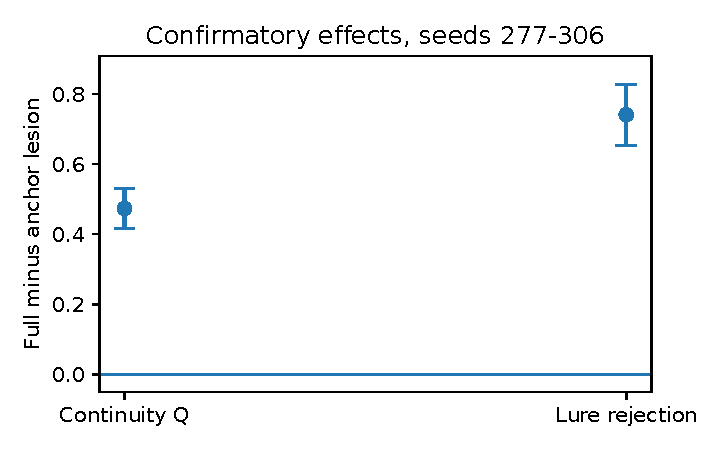
\includegraphics[width=\columnwidth]{confirmatory_effects_rerun.pdf}
\caption{Fresh confirmatory Full-minus-anchor-lesion effects on seeds 277--306. Error bars are paired-seed 95\% confidence intervals.}
\label{fig:heldout}
\end{figure}

The old-appearance lure captured the prior lineage in $0.035$ of Full probe frames and $0.775$ after lesion. Expressed as a positive Full advantage in lure rejection,
\begin{equation}
\Delta(1-L)=+0.740,\qquad95\%\;\mathrm{CI}=[0.653,0.828],
\end{equation}
with $d_z=3.16$, 30/30 seed-level wins, and positive direction in all four profiles. Continuity advantages ranged from $+0.331$ to $+0.594$ across profiles, while lure-rejection advantages ranged from $+0.500$ to $+0.906$ (Fig.~\ref{fig:profiles}). Full $Q$ had no floor or ceiling degeneracy.

\begin{figure}[t]
\centering
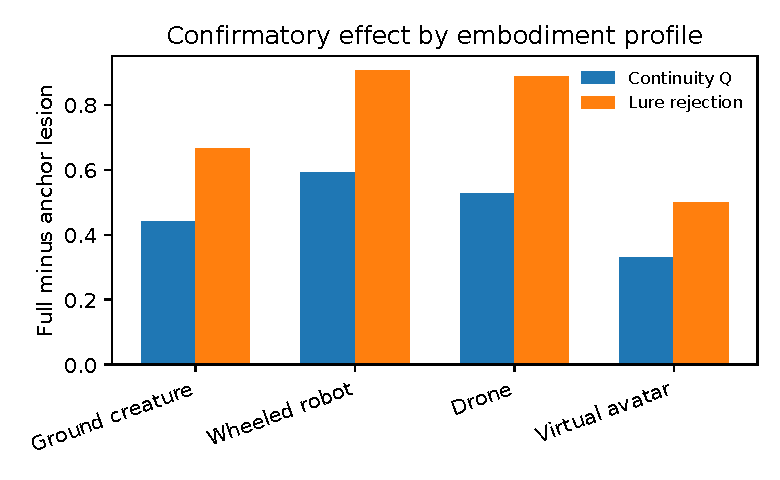
\includegraphics[width=\columnwidth]{embodiment_effects_rerun.pdf}
\caption{Confirmatory Full-model advantage by synthetic embodiment profile.}
\label{fig:profiles}
\end{figure}

\subsection{Independent recurrent estimator}
The independent-estimator held-out contains 30 fresh seeds, four profiles, and 120 matched scenes. CIAS Full attained mean final-probe identity continuity $0.948$ (95\% CI $[0.930,0.965]$) and lure capture $0.023$ ($[0.014,0.033]$). The generic recurrent estimator attained continuity $0.998$ and lure capture $0.0017$. On paired seed means, CIAS Full minus generic was $-0.0506$ for continuity (95\% CI $[-0.0676,-0.0345]$) and $-0.0218$ for lure rejection ($[-0.0314,-0.0130]$). Thus the independent estimator was slightly but consistently better on these two tracking metrics (Fig.~\ref{fig:generic}).

\begin{figure}[t]
\centering
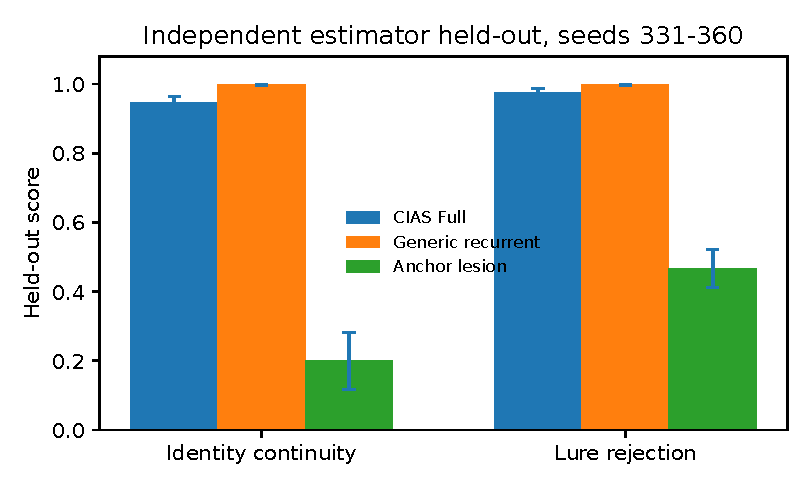
\includegraphics[width=\columnwidth]{independent_estimator_comparison.pdf}
\caption{Independent-estimator held-out on seeds 331--360. Lure rejection is $1-$lure capture. The generic recurrent estimator was fit only on diagnostic seeds 315--326 and was not retuned on preflight or held-out data.}
\label{fig:generic}
\end{figure}

The selected recurrent hyperparameters were motion weight $0.20$, appearance-continuity weight $0.00$, and state-update rate $0.10$. The selected recurrence therefore added no penalty for preserving visual appearance across frames. Current appearance components remained in the diagnostic-fitted Gaussian emission model together with the engineered causal-role features.

\subsection{Parameter sensitivity}
The 27-setting sensitivity experiment used seeds 361--390, separate from both earlier held-out ranges. Both Full-versus-lesion effect signs were preserved in 25/27 settings (92.6\%); the same 25 settings had both pointwise descriptive 95\% bootstrap intervals above zero and the expected direction in at least three of four profiles. Under the simultaneous max-bootstrap interval spanning all 54 sensitivity effects, 24/27 settings (88.9\%) retained positive lower bounds for both primary effects. The additional setting that lost simultaneous support was \texttt{joint\_04}: its identity advantage was $+0.082$, with a simultaneous lower bound of $-0.029$. Median identity-continuity advantage was $+0.760$ and median lure-rejection advantage $+0.524$. The weakest lure-rejection effect remained positive at $+0.211$. Identity continuity failed in two settings: a persistent-reconnect gate of 0.77 produced $-0.021$ with a confidence interval crossing zero, and one joint perturbation produced $-0.248$ with a fully negative interval. Figure~\ref{fig:sensitivity} shows the tested basin and these failure regions.

\begin{figure}[t]
\centering
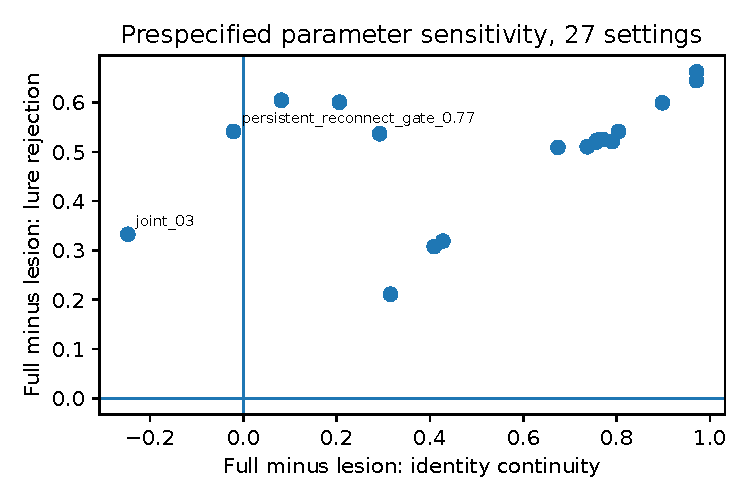
\includegraphics[width=\columnwidth]{parameter_sensitivity_basin.pdf}
\caption{Prespecified parameter sensitivity on seeds 361--390. Each point is one of 27 settings. Twenty-five settings remain in the positive-positive quadrant. The two labeled settings lose the identity-continuity advantage.}
\label{fig:sensitivity}
\end{figure}

\section{Negative Results and Theory Reduction}
The initial diagnostic reproduced the original ceiling failure: the legacy endpoint was exactly 1.0 in all conditions and could not discriminate the mechanism. The repaired diagnostic removed this ceiling and again failed to support a privileged progressive morphology sequence. Full progressive minus final-from-start was $+0.0147$ (95\% CI $[-0.0038,0.0331]$), minus reverse $+0.0071$ ($[-0.0041,0.0183]$), and minus random $+0.0051$ ($[-0.0124,0.0225]$). Progressive order is therefore excluded from the supported core theory.

The history-reset control further separates final local attribution from persistent lineage. On the confirmatory rerun, history reset reached $Q=0.874$ versus $0.883$ for Full; Full-minus-reset was only $+0.009$ (95\% CI $[-0.005,0.023]$). Lure capture was likewise close: 0.048 after history reset and 0.035 in Full. Yet the lineage diagnostics differed qualitatively. Full preserved the stage identity chain and retained the initial identity at the end of every run, whereas history reset had stage-chain score 0 and initial-identity retention 0. Whole-run Self fragmentation averaged 2.08 for Full and 4.24 after history reset. The composite final-probe score can therefore be high after local re-identification even when the original cross-stage lineage has been discarded. Persistent lineage and amount of retained association history are separable state variables.

The independent recurrent estimator provides a second theory reduction. It outperformed CIAS Full on the additional held-out tracking metrics while containing no explicit persistent-Self variable or reconnect rule. The data reject architectural uniqueness of the explicit anchor. Both successful solutions integrate multichannel observations across time, and the recurrent estimator selected zero additional appearance-continuity penalty. Its emission model still contains current appearance features, so this comparison does not isolate causal-role cues as sufficient by themselves.

The supported core is most conservatively summarized as
\begin{equation}
\boxed{\begin{aligned}
\text{persistent functional identity}\;\Leftarrow\;&\;\text{causal individuation}\\
&+\text{embodied closure}\\
&+\text{cross-time state}
\end{aligned}}
\label{eq:core}
\end{equation}
where the cross-time state may be implemented by an explicit persistent anchor, as in CIAS, or implicitly by a generic recurrent estimator. Equation~\eqref{eq:core} is a functional summary, not an arithmetic identity or a claim of uniqueness.

\section{Discussion}
The confirmatory rerun establishes a strong causal role for the persistent anchor inside CIAS. Selective removal reduces the composite continuity score by 0.473 and increases old-body lure capture from 0.035 to 0.775. The error is specifically a lineage error. Without the cross-change anchor, the ontology frequently follows the entity that preserves the old appearance/location pattern. The transformed body simultaneously carries the stronger current causal relation.

The independent estimator changes the interpretation of that lesion. A supervised recurrent state estimator with no Self role, no persistent lineage key, and no change-point reconnect rule attained nearly perfect held-out tracking, so the benchmark does not require an explicit anchor. Diagnostic model selection assigned zero weight to the additional recurrent appearance-continuity term, while current appearance remained in the fitted emission model. The result supports temporally integrated multichannel evidence and rejects the stronger architecture-level uniqueness claim. The persistent anchor is an interpretable mechanism for carrying identity through a discontinuity; a generic recurrent estimator can encode an equivalent functional state implicitly.

The benchmark separates two questions: which information supports persistent identity, and which architecture stores that information? The present evidence shows that multichannel observations integrated across time can sustain identity after visual discontinuity. The generic estimator's zero recurrent appearance-continuity weight indicates that explicit preservation of visual similarity across frames was unnecessary in its selected configuration, although current appearance remained one emission feature. Several storage mechanisms remain compatible with the evidence. Explicit anchors are inspectable, directly lesionable, and can be tied to autobiographical ownership; generic recurrent state may offer better tracking while making the represented identity variable less explicit.

The history-reset control separates final local attribution from cross-stage lineage. After association history is cleared, final-probe $Q$ recovers to a value close to Full, while the original lineage is lost and whole-run fragmentation increases. Complete autobiographical association history is therefore unnecessary for high final-probe attribution, and final local attribution alone does not establish preservation of the original lineage. This motivates reporting both local tracking metrics and explicit cross-stage lineage metrics.

The sensitivity experiment constrains the role of the numerical constants. The nominal mechanism lies within a finite local operating basin: 25 of 27 prespecified perturbations preserve both Full-versus-lesion effects with positive pointwise intervals, and 24 remain jointly positive under the family-wise max-bootstrap interval across all 54 sensitivity effects. Increasing the persistent reconnect gate to 0.77 eliminates the identity advantage, and one joint perturbation reverses it. These failure regions identify a critical boundary: if reconnection becomes too difficult after a discontinuity, the explicit lineage state ceases to provide a continuity benefit.

The results connect to sensorimotor self/other models \cite{Lanillos2017,Lanillos2020,Oliver2022,Chen2026}, learned and adaptive body models \cite{Bongard2006,Hu2025}, object-file accounts of temporal persistence \cite{Kahneman1992}, and state-estimation approaches \cite{Kalman1960,Rabiner1989,Kaelbling1998}. The contribution is a controlled causal study of identity information and cross-time state under adversarial embodiment change. Unique necessity of a Self-specific data structure is unsupported by the independent-estimator experiment.

\section{Limitations}
\noindent\emph{Engineered representation.} The benchmark uses semantically engineered causal variables. The generic estimator is also trained on those features and uses diagnostic lineage labels to fit its emission model. Neither experiment shows how Self-relevant causal variables emerge from pixels, tactile streams, or unsupervised experience. End-to-end causal representation learning \cite{Scholkopf2021} and physical-sensor transfer remain necessary tests.

\noindent\emph{Comparator scope.} The recurrent baseline is one supervised state estimator. HMM/POMDP estimators, probabilistic filters with explicit uncertainty, deep association trackers, and transformer memories remain untested. The experiment rejects uniqueness of the explicit CIAS anchor in this benchmark. The optimal generic architecture remains undetermined.

\noindent\emph{Parameter domain.} The 27-setting sweep maps a broad finite neighborhood around the tested mechanism. Two settings failed the identity-continuity criterion. The result therefore concerns this finite neighborhood; many coefficient combinations remain untested. Endpoint weights were held fixed because this sweep targeted behavior-affecting mechanism parameters.

\noindent\emph{Task and embodiment scope.} The activity inside each embodiment is minimal sensorimotor probing without navigation, manipulation, social interaction, or long-horizon planning. The four profiles are synthetic reliability/noise regimes and do not constitute four physical morphology transfers. The lure and causal signals are generated by a benchmark designed around the identity question, so ecological validity and adversarial transfer to richer worlds remain open.

\noindent\emph{Functional scope.} The term Self denotes a computationally individuated subject variable. The experiments measure persistent identity assignment and lineage under controlled causal conflict. They provide no evidence of qualia, phenomenal consciousness, human-like self-awareness, or moral status.

\section{Conclusion}
A fresh end-to-end rerun reproduced the central CIAS lesion result: on 30 untouched confirmatory seeds, selective removal of the persistent causal identity anchor reduced $Q$ from 0.883 to 0.410 and increased old-body lure capture from 0.035 to 0.775. The effect was large, nondegenerate, and present in all four synthetic embodiment regimes. A separate 27-setting held-out sensitivity experiment preserved both Full-versus-lesion effects with positive pointwise intervals in 25 settings; 24 remained positive for both effects under a simultaneous family-wise max-bootstrap interval, showing a substantial operating basin together with identifiable failure regions.

The independent recurrent estimator supplies the critical qualification. Given the same structured observations and diagnostic supervision, a generic temporal state estimator slightly outperformed CIAS Full on separate held-out tracking metrics. Its selected recurrent configuration used no additional appearance-continuity penalty, although appearance components remained in the emission model. The benchmark therefore does not require an explicit Self anchor. CIAS implements cross-time identity with an explicit, interpretable lineage anchor; recurrent state estimation can carry functionally equivalent continuity state implicitly.

The resulting theory is narrower than an architectural necessity claim and broader than one mechanism. Persistent functional identity in the present setting depends on causal individuation, embodied closure, and a cross-time state that survives appearance discontinuity. The precise representation of that state remains an empirical design question. Learning the relevant causal variables from raw sensors, testing richer physical embodiments, and comparing additional generic estimators are the next steps. Phenomenal consciousness remains outside the evidence.

\section*{Data and Code Availability}
The public reproducibility repository contains the executable scientific core, complete diagnostic and confirmatory rerun, independent-estimator experiment, 27-setting parameter-sensitivity experiment, analysis code, seed ledgers, reference results, and SHA-256 provenance: \url{https://github.com/NicholasShatokhin/cias-persistent-functional-self}. The reference execution used Godot 4.7 stable. The canonical core SHA-256 is
\begin{center}
\small\texttt{b81f43221b290fc09c06c69719a24533}\\
\texttt{cdd802fe483347301d6015adda9eb38c}.
\end{center}
The complete rerun is prepared as a versioned repository release for immutable Zenodo archival \cite{CIASRepo2026}. The release DOI token \texttt{ZENODO-CURRENT-RELEASE-DOI} is replaced with the newly assigned Zenodo version DOI before final submission. The preceding DOI 10.5281/zenodo.22207678 remains the historical confirmatory snapshot.

\section*{Acknowledgment}
This research received no external funding. The author declares no competing interests. In accordance with IEEE policy, the author discloses the use of OpenAI ChatGPT (GPT-5.6 Sol) as an AI-assisted research and writing tool. It assisted with drafting and restructuring prose and with generation/review of portions of experimental and analysis code. The author selected the research questions, executed the reported experiments, inspected the data and outputs, verified the cited literature and mathematical claims, made all scientific decisions, and takes full responsibility for the submitted content.

\bibliographystyle{IEEEtran}
\bibliography{references}
\end{document}
